\documentclass[12pt]{article}
\usepackage{graphicx}
\usepackage{amsmath}

\begin{document}
CSCI-4100 Assignment 7\\
Yichuan Wang \\
RIN:661414395\\\\
1. (500) Classifying Handwritten Digits: 1 vs. 5\\
Linear regression followed by pocket algorithm improvement is used in this problem.\\
Math definition for feature 1 (normalized y-axis asymmetry):\\
$$\frac{1}{256}\sum_{i=0}^{15}\sum_{j=0}^7|pix[i][j]-pix[i][15-j]|$$
Math definition for feature 2 (normalized x-axis asymmetry):\\
$$\frac{1}{256}\sum_{i=0}^7\sum_{j=0}^{15}|pix[i][j]-pix[15-i][j]|$$
Normalization is required since original feature values are too large and will make linear regression result too small to play a role.\\
For all the plots below, feature 1 is horizontal axis, and feature 2 is vertical axis.\\
(a) \\%DONE
The training output $[g_0...g_d]$ is $$[1.2215, -4.2678, -3.1657]$$
Training data result:\\
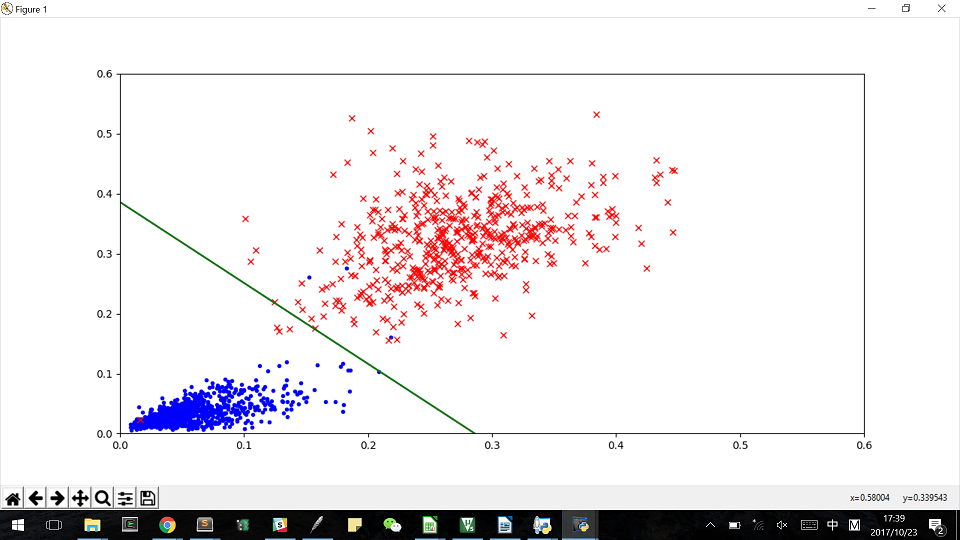
\includegraphics[scale=0.6]{image/linear_train}\\\\
Test data result:\\
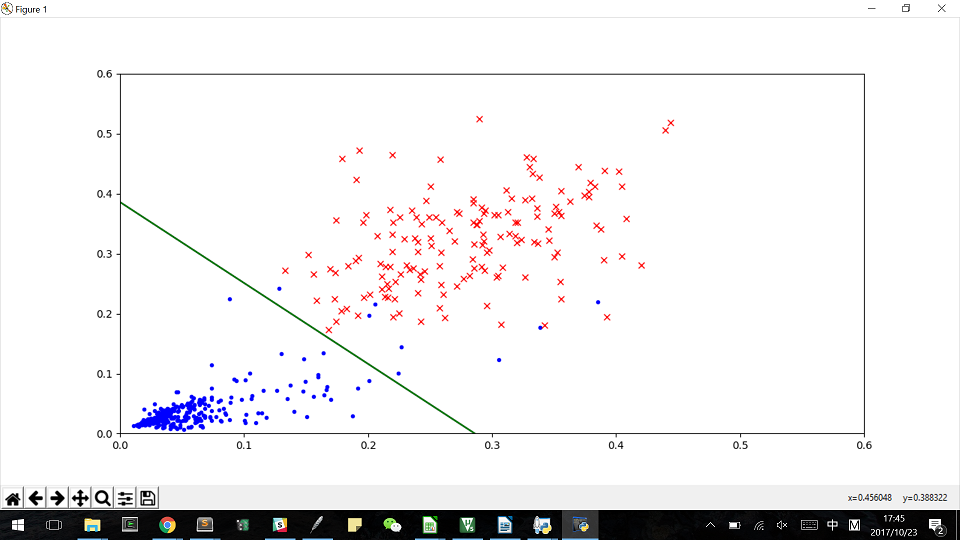
\includegraphics[scale=0.6]{image/linear_test}\\\\
(b)\\%DONE
Error Calculation:
The error calculation is done in the software, the result is given here:\\
$$E_{in}=0.0045$$
$$E_{test}=0.0189$$\\
(c)\\%DONE
Error bound calculation:
$$E_{out} \leq  E_{in}+\sqrt{\frac{8}{1561}ln(\frac{4\times ((1561\times 2)^{3}+1)}{0.05})} = 0.0045+0.3823 = 0.3868$$
$$E_{out} \leq  E_{test}+\sqrt{\frac{1}{2\times424}ln(\frac{1\times 2}{0.05})} = 0.0189+0.0660 = 0.0849$$
The bound based on $E_{test}$ is a better bound.\\\\
(d)\\%DONE
The 3rd-order transform is performed as following:
$$[x_0,x_1,x_2]\longrightarrow [x_0, x_1, x_2, x_1^2 ,x_2^2, x_1x_2, x_1^3, x_2^3, x_1^2x_2, x_1x_2^2]$$
The training output $[g_0...g_d]$ is $$[1.0567, 2.8568, -4.4757, -10.6157, -4.8360, -36.8246, 18.9741, 3.1472, -0.3295, 83.0706]$$
Training data result: $E_{in}=0.0026$\\
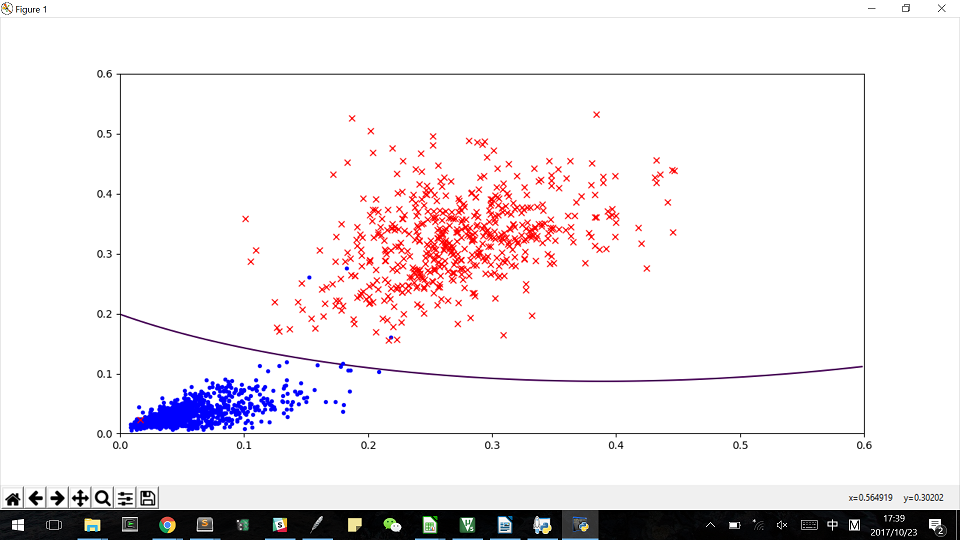
\includegraphics[scale=0.6]{image/3rd_train}\\\\
Test data result: $E_{test}=0.0213$\\
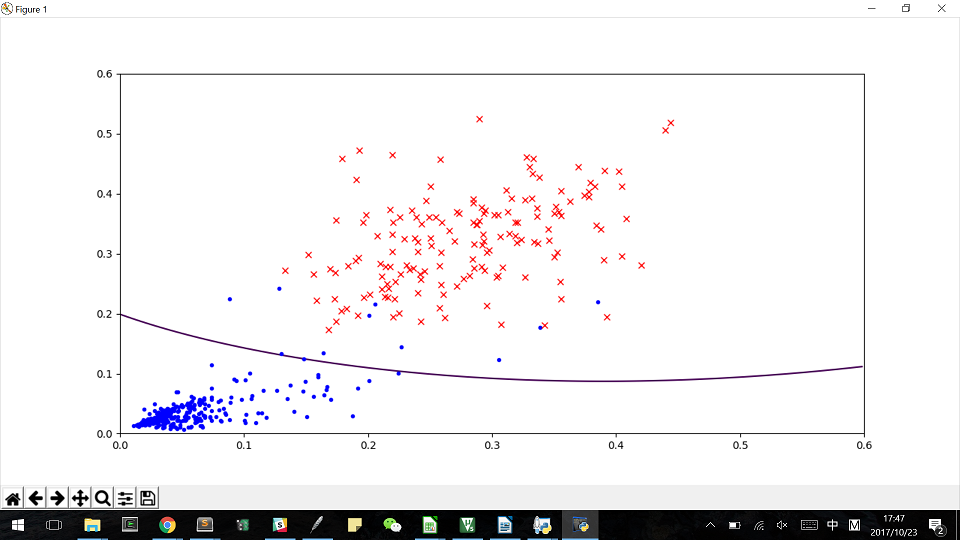
\includegraphics[scale=0.6]{image/3rd_test}\\\\
Error bound calculation:
$$E_{out} \leq  E_{in}+\sqrt{\frac{8}{1561}ln(\frac{4\times ((1561\times 2)^{10}+1)}{0.05})} = 0.0026+0.6594 = 0.6620$$
$$E_{out} \leq  E_{test}+\sqrt{\frac{1}{2\times424}ln(\frac{1\times 2}{0.05})} = 0.0213+0.0660 = 0.0873$$
The bound based on $E_{test}$ is a better bound.\\\\
%DONE
(e) I would like to deliver the 2D-perceptron model instead of the 3rd-order-transform one. First of all, the 2D model has a better error bar; data is nearly separable in its original form. Second, the 3rd-order-transform model is much more complicated than the 2D model ($d_{vc}=3$ vs $d_{vc}=10$), and a over complicated model is likely to fit more noise.\\\\
2. (200) Gradient Descent on a "Simple" Function\\%DONE
(a) Original Function: $f(x)=x^2+2y^2+2sin(2\Pi x)sin(2\Pi y)$
$$\frac{df(x)}{dx}=2x+4\Pi cos(2\Pi x)sin(2\Pi y)$$
$$\frac{df(x)}{dy}=4y+4\Pi sin(2\Pi x)cos(2\Pi y)$$
Gradient Decent result:\\
$\eta=0.01$\\
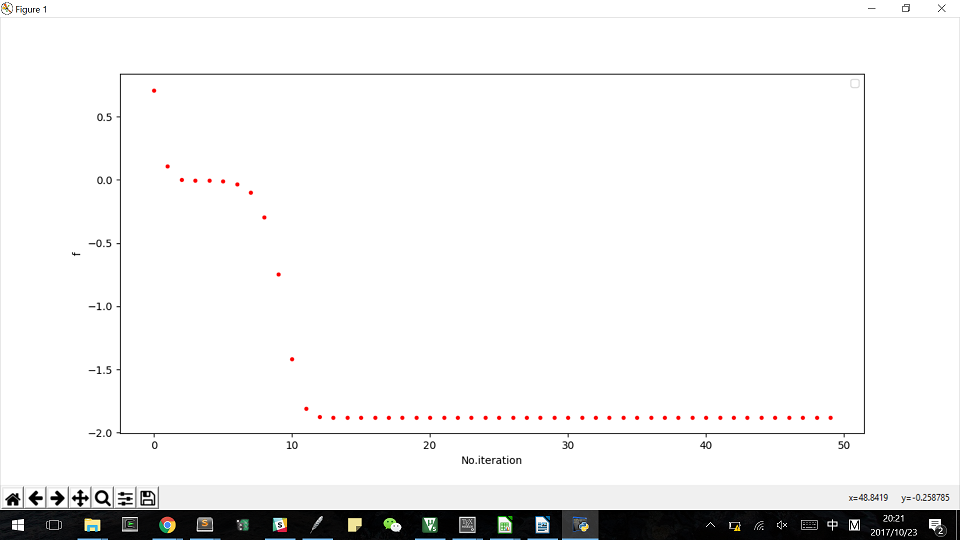
\includegraphics[scale=0.6]{image/0d01}\\\\
$\eta=0.1$\\
With $\eta=0.1$ the algorithm results in serious bouncing and cannot find the local minimum.\\
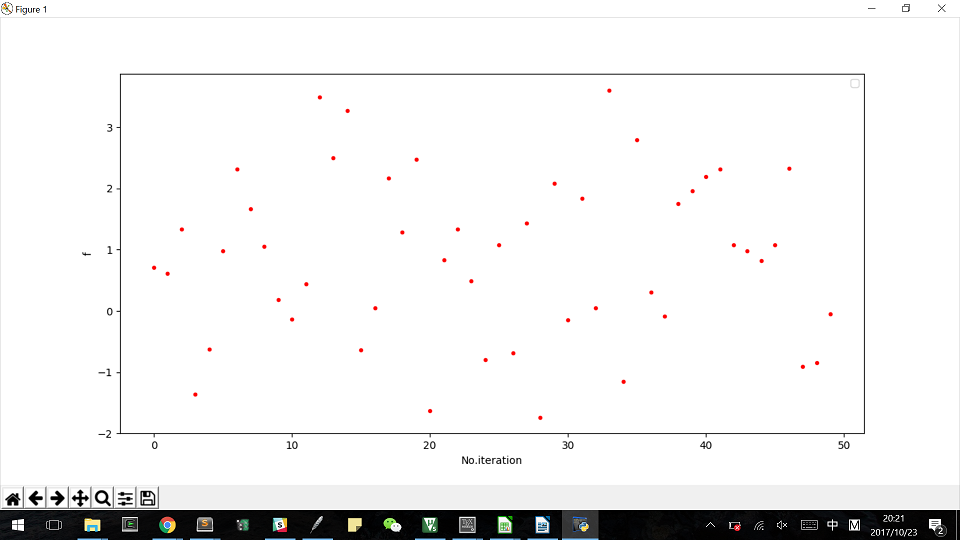
\includegraphics[scale=0.6]{image/0d10}\\\\
(b) Table:\\ %DONE
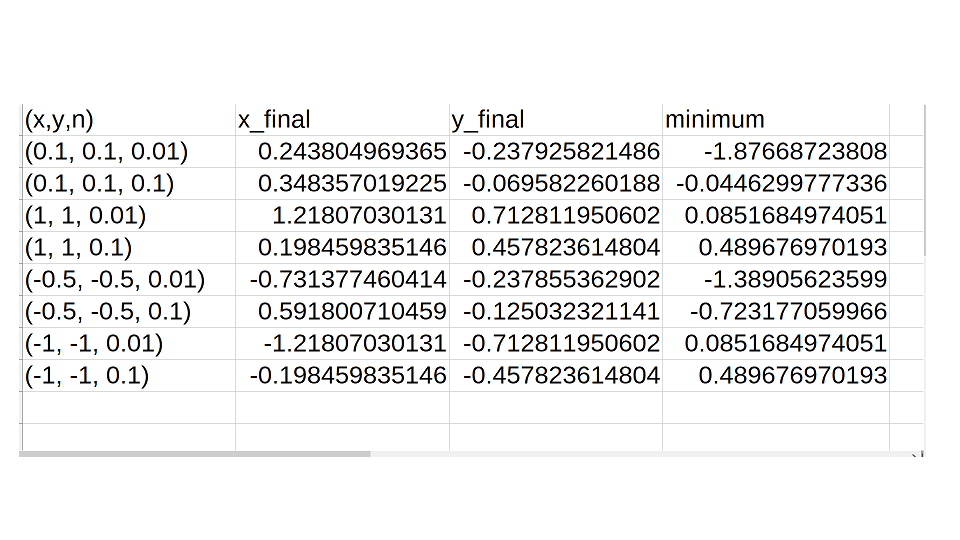
\includegraphics[scale=0.6]{image/table}\\
It is observed that different starting location gives different local minimum; it is hard to find a global minimum in such condition.\\\\
3. (300) Problem 3.16 in LFD\\
(a)%DONE
$$cost(accept) = P[correct]*0 + P[intruder]*C_a = (1-g(x))\times C_a$$
$$cost(reject) = P[correct]*C_r + P[intruder]*0 = g(x)\times C_r$$
(b) It's the trade off between accept and reject. When $cost(accept)\leq cost(reject)$ we will accept the person: %DONE
$$(1-g(x))\times C_a \leq g(x)\times  C_r $$
$$C_a-g(x)\times C_a \leq g(x)\times  C_r $$
$$C_a \leq g(x)\times  (C_r+C_a) $$
$$g(x) \geq \frac{C_a}{C_r+C_a} $$
$$k = \frac{C_a}{C_r+C_a} $$
(c)\\%DONE
Supermarket: $C_a=1$ $C_r=10$
$$k = \frac{1}{10+1} = 0.0909$$
CIA: $C_a=1000$ $C_r=1$
$$k = \frac{1000}{1000+1} = 0.9990$$
The intuition is that the supermarket has a high cost of false reject, so it will accept the person at a relatively low threshold. CIA has a high cost of false accept, so they accept the person only when they are super sure that it's the correct person, and thus has a high threshold.
\end{document}












